\subsection{Spacecraft cost}
	The spacecraft cost can be estimated depending on several parameters and criteria, such as the type of mission, the subsystem considered and the unit over which calculate the cost. In our specific case we concentrated on the cost analysis for a communication-type satellite and review it for every subsystem of the spacecraft and its launch procedure.\\

	The subsystems analysed  are the following:
	\begin{itemize}
		\item Attitude determination and Control subsystem (ADCS)
		\item Communication subsystem
		\item Electrical power subsystem (EPS)
		\item Integration assembly and test (IA\&T)
		\item Passive sensor
		\item Propulsion
		\item System engineering
		\item Structure
		\item Thermal control
		\item Telemetry tracking and command (TT\&C)
	\end{itemize}
	In particular, \autoref{fig:torta} shows the cost percentage that each system represents: from it we can see that the System Engineering is the most important item, followed by the \gls{eps} and the IA\&T subsystems. Moreover, \autoref{fig:distribution} lists the different sections, depending on the type of mission the satellite is intended to 					accomplish, with their standard deviations; tables \ref{fig:mission} and \ref{fig:mission_pound}, instead, show the total cost depending on the mission type and the total cost per pound \cite{Fox2008}.

	\begin{figure}
		\centering
		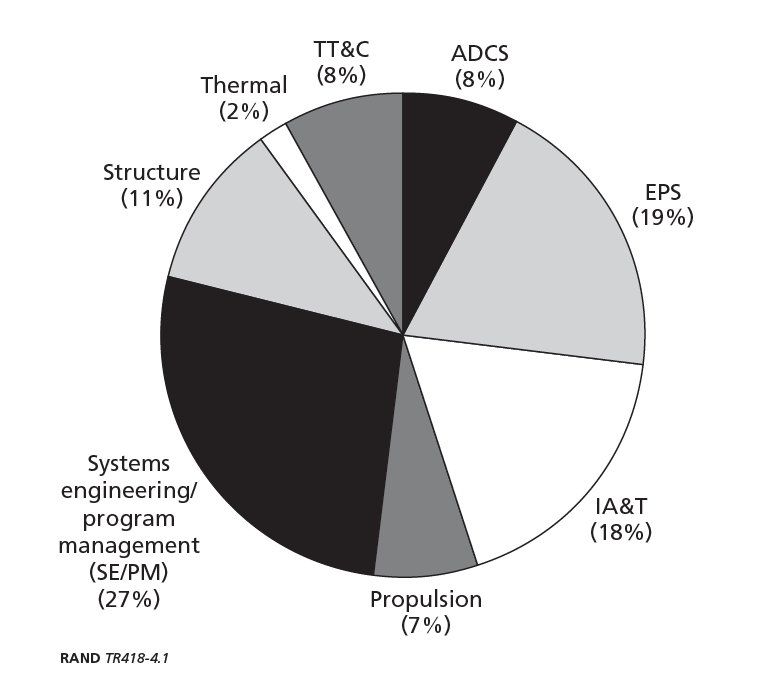
\includegraphics[width = .7\textwidth]{Torta.png}
		\caption{Communication spacecraft cost composition}
		\label{fig:torta}
	\end{figure}

	\begin{figure}
		\centering
		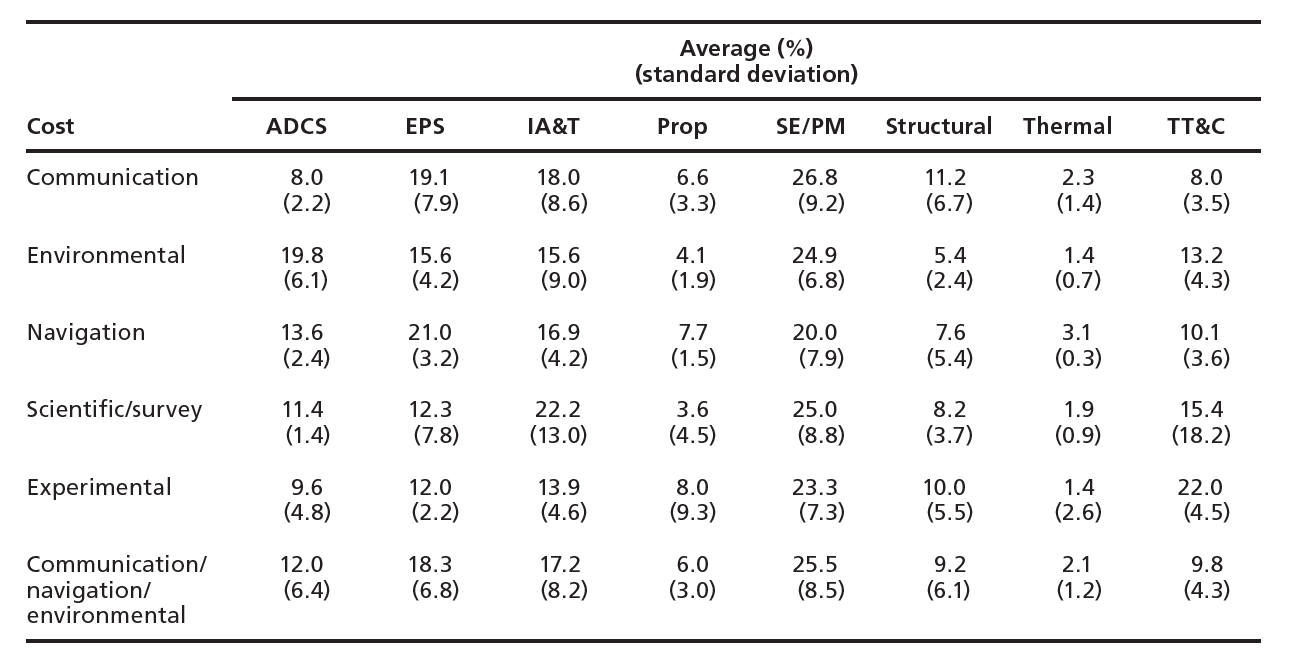
\includegraphics[width = 1\textwidth]{Standard_dev.png}
		\caption{Communication spacecraft cost composition: averages and standard deviations}
		\label{fig:distribution}
	\end{figure}

	\begin{figure}
		\centering
		\begin{minipage}{1\textwidth}
		\centering
		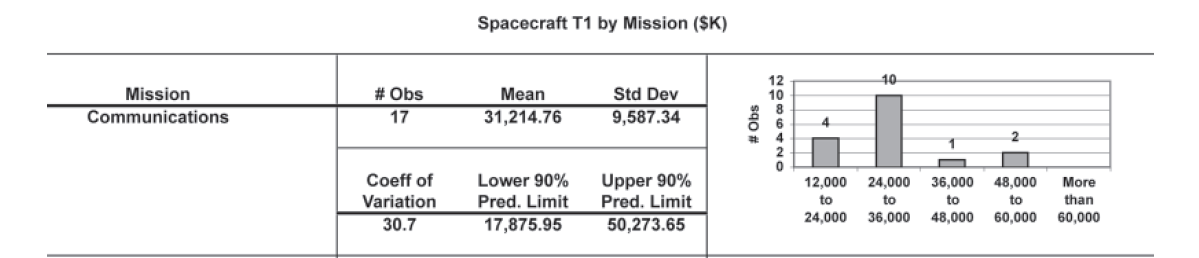
\includegraphics[width = .95\textwidth]{Mission.png}
		\caption{Total spacecraft cost}
		\label{fig:mission}
		\end{minipage}
		\hspace{20mm}
		\begin{minipage}{.95\textwidth}
		\centering
		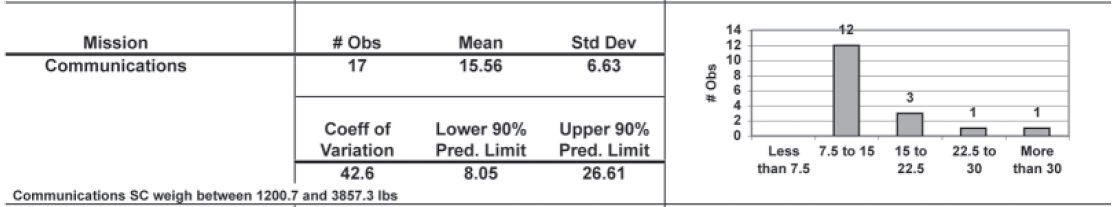
\includegraphics[width = .95\textwidth]{Mission_pound.png}
		\caption{Total spacecraft cost per pound}
		\label{fig:mission_pound}
		\end{minipage}
	\end{figure}

	Regarding the cost per subsystem, \autoref{tab:systems1} and \autoref{tab:systems2} show the different cost each subsystem is intended to have:

	\begin{table}
		\centering
		\begin{tabular}{ccc}
		\toprule
		Subsystem & Mean Cost (k\euro) & Standard deviation\\
		\midrule
		IA\&T     & 8311,49   & 8719,94\\
		EPS        & 8441,34   & 5681,80\\
		Structure & 4111,49   & 2955,92\\
		SEPM      & 12167,05 & 7825,63\\
		Thermal  & 903,45    & 562,3\\
		TT\&C    & 4423,24   & 2942,24\\
		\bottomrule
		\end{tabular}
		\caption{List of the costs per subsystem}
		\label{tab:systems1}
	\end{table}

	\begin{table}
		\centering
		\begin{tabular}{ccc}
		\toprule
		Subsystem & Mean Cost/unit (k\euro/kg or ch) & Standard deviation\\
		\midrule
		ADCS                                         & 94,70     & 8719,94\\
		Communication ($1 < ch < 10$)   & 3923,19 & 1443,98\\
		Communication ($10 < ch < 25$) & 1534,45 & 558,37\\
		Communication ($25 < ch$)         & 708,40   & 197,35\\
		EPS                                            & 24,7      & 7,27\\
		Propulsion                                  & 54,68     & 14,32\\
		Structure                                    & 15,94     & 4,37\\
		\bottomrule
		\end{tabular}
		\caption{List of the costs per subsystem per pound/channel}
		\label{tab:systems2}
	\end{table}

	Through this data we can make a raw hypothesis on the average total cost of the spacecraft with a summary estimation of its mass:

	\begin{table}
		\centering
		\begin{tabular}{ccc}
		\toprule
		\multicolumn{3}{c}{Communication spacecraft}\\
		\midrule
		IA\&T       & 8311,49 \euro       & $+$\\
		EPS          & 24,7 \euro/Kg        & $\times 604,92 +$\\
		Structure   & 4111,5 \euro     & $+$\\
		SEPM        & 12167,05 \euro     & $+$\\
		Thermal    & 903,45 \euro        & $+$\\
		TT\&C       & 4423,24 \euro      & $+$\\
		ADCS        & 94,70 \euro/Kg     & $\times 27,52 +$\\
		Propulsion & 54,68   \euro/Kg   & $\times 3550 +$\\
		Communication ($10 < ch < 25$) & 1534,45 \euro/ch & $\times 12 ch =$\\
		\bottomrule
		Total cost:& & 259.991.798 \euro\\
		\end{tabular}
		\caption{List of the costs per subsystem per pound/channel}
		\label{tab:cost}
	\end{table}
\subsection{Launch cost}
For the launch cost we based our considerations on the prices listed by the $SpaceX$ company. \autoref{fig:spacex} shows the prices for different types of launches, depending on the mass of the spacecrafts and the orbits they should reach \cite{spacex}.

Through the considerations we made in the previous sections we can state that around $124$ Millions of dollars ($105.124.400$ \euro) are needed for the launch: in fact each spacecraft has a total mass of about 3138,54 kg and the Molniya orbit is a HEO orbit; moreover, since the raans of the two orbital planes are separated of 180 $\deg$ it is necessary to use two separate launchers, one for each spacecraft.\\

Through this analysis the total cost for the project is:
\begin{equation}
Cost_{Total} = Cost_{Launch} + Cost_{Spacecraft} =  365.116.198 \text{ \euro}
\end{equation}

\begin{figure}[htbp]
\centering
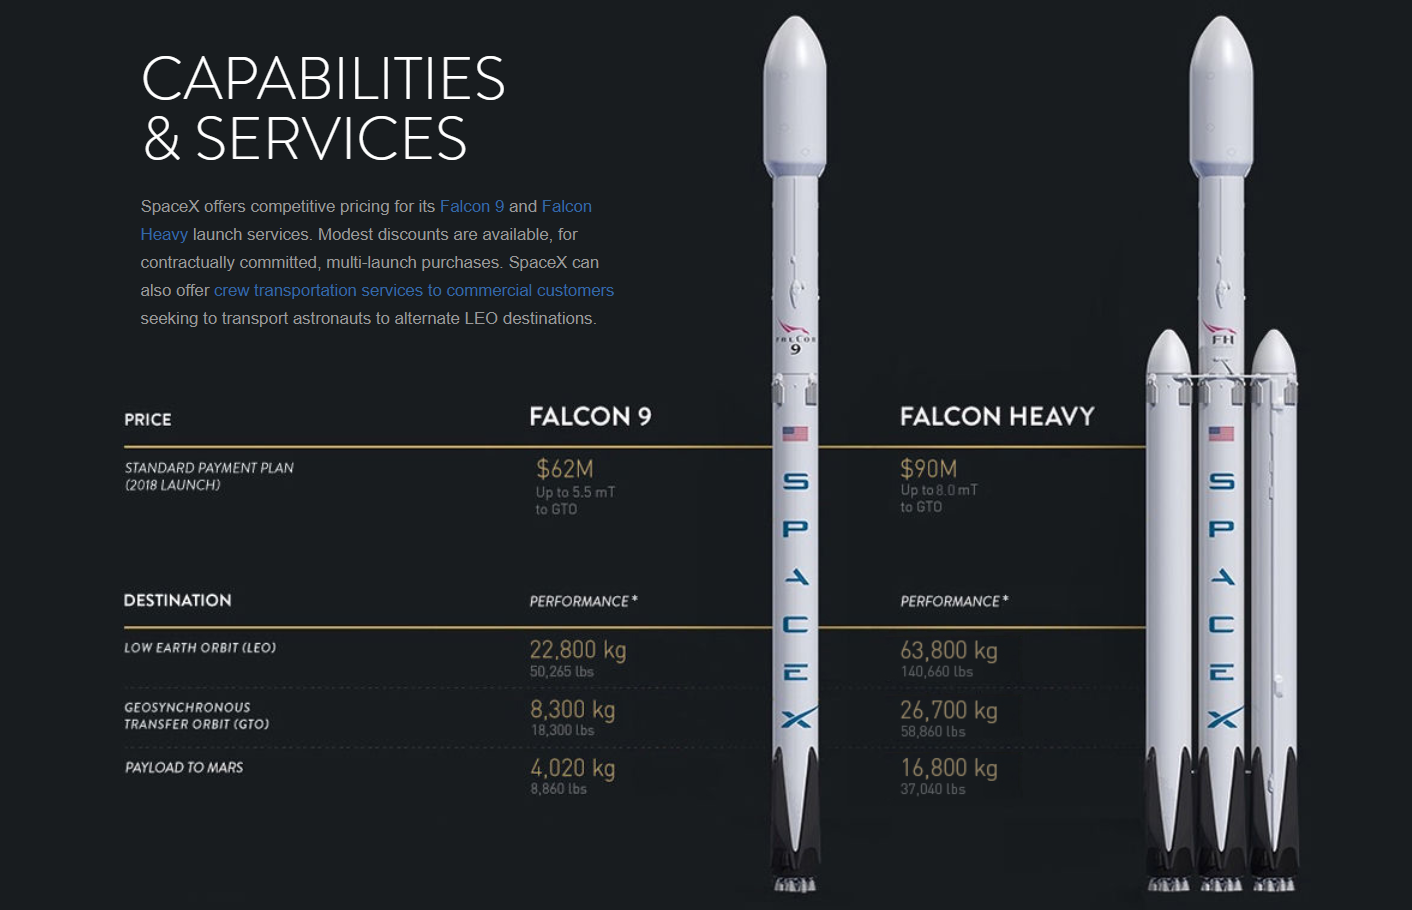
\includegraphics[width = .8\textwidth]{Spacex.png}
\caption{$SpaceX$ price list}
\label{fig:spacex}
\end{figure}
